\chapter{ПРАКТИКО-ОРИЕНТИРОВАННЫЕ ЗАДАЧИ}
\section{Текстовые задачи}


\textbf{2422.} $54 \cdot \frac{135}{100} = 54. \cdot 1,35 = 72,9$ \newline \null \hspace*{\fill} Ответ: 72,9.

\textbf{2423,2424.} Аналогичные задачи.

\textbf{2425.} $40 \cdot \frac{80}{100} = 32.$ \newline \null \hspace*{\fill} Ответ: 32.

\textbf{2426.} Аналогичная задача.

\textbf{2427.} $350 \cdot \big( 1+\frac{12}{100}\big) = 350 \cdot 1,12 = 392$. \newline \null \hspace*{\fill} Ответ: 392. 

\text{Замечание. Увеличение некоторой величины на } $p\%,$\newline\text{соответствует ее умножению на } $1 + \frac{p}{100};$\text{ уменьшение величины}\newline{на }$q$ \text{ее умножению на } $1 - \frac{q}{100}.$

\textbf{2428-2431.} Аналогичные задачи.

\textbf{2432.} $28 \cdot 1,1 = 30,8.$ \newline \null \hspace*{\fill} Ответ: 30,8. 

\textbf{2433-2436.} Аналогичные задачи.

\textbf{2437.} $\text{40 млн. руб.} \cdot \frac{25}{100} = \text{10 млн. руб.}$ \newline \null \hspace*{\fill} Ответ: 10 000 000. 

\textbf{2438-2441.} Аналогичные задачи.

\textbf{2442.} \text{Частные акционеры получат 20\% прибыли, т.е.} \newline $70 \text{млн. руб.}\cdot \frac{20}{100} = 14 \text{млн. руб.} $ \newline \null \hspace*{\fill} Ответ: 14 000 000. 

\textbf{2443-2446.} Аналогичные задачи. 

\textbf{2447.} $500 \cdot 1,11 = 555.$ \newline \null \hspace*{\fill} Ответ: 555. 

\textbf{2448-2451.} Аналогичные задачи. 

\textbf{2452.} $\text{Если } S \text{ первоначальная цена товара, то } S \cdot \big(1 - \frac{50}{100}\big)=940,$ \newline\text{ откуда }$ S = 940 \cdot 2 = 1880.$ \newline \null \hspace*{\fill} Ответ: 1880. 

\textbf{2453-2456.} Аналогичные задачи. 

\textbf{2457.} $8 \cdot 2000 \cdot \big(1 - \frac{5}{100}\big) = 8 \cdot 2000 \cdot 0,95 = 15200.$ \newline \null \hspace*{\fill} Ответ: 15200. 

\textbf{2428-2461.} Аналогичные задачи. 

\textbf{2462.} $200 \cdot \big(1 + \frac{p}{100}\big)=230;\enspace 200 + 2p = 230;\enspace p=15.$ \newline \null \hspace*{\fill} Ответ: 15. 

\textbf{2463-2466.} Аналогичные задачи. 

\textbf{2467.} $150 \cdot \big( 1 - \frac{p}{100}\big)=120;\enspace 150 - 1,5p = 120;\enspace p=20.$ \newline \null \hspace*{\fill} Ответ: 20. 

\textbf{2468-2470.} Аналогичные задачи.

\textbf{2471.} $70 \cdot \big(1 - \frac{p}{100}\big)=65,1;\enspace 70 - 0,7p = 65,1;\enspace p = 7.$ \newline \null \hspace*{\fill} Ответ: 7. 

\textbf{2472-2474.} Аналогичные задачи.

\textbf{2475.} $2200 \cdot \big(1 - \frac{p}{100}\big) = 1100;\enspace 2200 - 22p = 1100;\enspace p = 50.$ \newline \null \hspace*{\fill} Ответ: 50. 

\textbf{2476-2478.} Аналогичные задачи.

\textbf{2479.} $S = 600 \cdot \big( 1 -\frac{45}{100}\big)\cdot\big( 1 - \frac{10}{100}\big) = 600 \cdot 0,55 \cdot 0,9 = 297.$ \newline \null \hspace*{\fill} Ответ: 297. 

\textbf{2480-2482.} Аналогичные задачи.

\textbf{2483.} $1100 \cdot \big( 1 - \frac{p}{100}\big) = 869;\enspace 1100 - 11p = 869;\enspace p = 21.$ \newline \null \hspace*{\fill} Ответ: 21. 

\textbf{2484, 2485.} Аналогичные задачи.

\textbf{2486.} $300 + 300 \cdot \big(1 - \frac{80}{100}\big) = 300 + 60 = 360.$ \newline \null \hspace*{\fill} Ответ: 360. 

\textbf{2487, 2488.} Аналогичные задачи.

\textbf{2489.} $2 \cdot 132 + 16 \cdot 132 \cdot \big( 1 -\frac{50}{100}\big) = 264 + 1056 = 1320.$ \newline \null \hspace*{\fill} Ответ: 1320. 

\textbf{2490, 2491.} Аналогичные задачи.

\textbf{2492.} $1 - \frac{p}{100} = 0,98;\enspace p = 2.$ \null \hspace*{\fill} Ответ: 2. 

\textbf{2493, 2494.} Аналогичные задачи.

\textbf{2495.} $104 \cdot \frac{8}{5+8} = 104 \cdot \frac{8}{13} = 64.$ \newline \null \hspace*{\fill} Ответ: 64. 

\textbf{2496-2498.} Аналогичные задачи.

\textbf{2499.} $\text{96 млн. руб.}\cdot \frac{3}{3+5} = \text{36 млн. руб.}.$ \newline \null \hspace*{\fill} Ответ: 36 000 000. 

\textbf{2500-2502.} Аналогичные задачи.

\textbf{2503.} $\text{Интересуются футболом } 210000 \cdot \big( 1 - \frac{1}{6}\big) = 175000 \text{ человек,}$\newline\text{из них матч смотрели }$ 175 000 \cdot \frac{5}{7} = 125 000 \text{ человек.}$\newline\text{Не посмотрело этот матч }$ 210000 - 125000 = 85000 \text{ человек }.$ \newline \null \hspace*{\fill} Ответ: 85000. 

\textbf{2504-2506.} Аналогичные задачи.

\textbf{2507.} $\text{Если } x \text{ первоначальное число шариков, то продано их}$\newline$\text{было }\frac{3x}{8} + 15 \text{ штук, а осталось }\frac{x}{4}.\text{ Поэтому } x = \frac{3x}{8} + 15 + \frac{x}{4}, \text{ откуда}$\newline$ x = 40.$ \newline \null \hspace*{\fill} Ответ: 40.  

\textbf{2508-2510.} Аналогичные задачи.

\textbf{2511.} $\text{Лиственные деревья составляют } \frac{19}{1+19} = \frac{19}{20} \text{ часть всех}$\newline$\text{деревьев, что в процентном соотношении составляет } \frac{19}{20} \cdot 100, \text{ т.е. }$\newline$ 95\%$. \newline \null \hspace*{\fill} Ответ: 95. 

\textbf{2512-2514.} Аналогичные задачи.

\textbf{2515.} $108 \cdot \frac{5}{7+5} = 108 \cdot \frac{5}{12} = 45.$ \newline \null \hspace*{\fill} Ответ: 45. 

\textbf{2516-2518.} Аналогичные задачи.

\textbf{2519.} $\frac{1}{1+24} \cdot 100\% = 4\%.$ \null \hspace*{\fill} Ответ: 4. 

\textbf{2520-2522.} Аналогичные задачи.

\textbf{2523.} $11 \text{ минут это } 11 \cdot 60 = 660 \text{ секунд, за это время принтер}$\newline\text{напечатает } $\frac{660}{6} = 110 \text{ страниц}.$ \newline \null \hspace*{\fill} Ответ: 110. 

\textbf{2524-2526.} Аналогичные задачи.

\textbf{2527.} $\frac{1,7 \cdot 10^7}{9,5 \cdot 10^6} = \frac{17}{9,5} \approx 1,79.$ \newline \null \hspace*{\fill} Ответ: 2. 

\textbf{2528-2530.} Аналогичные задачи.

\textbf{2531.} $\frac{5,9 \cdot 10^7}{5,4 \cdot 10^5}=\frac{590}{5,4}\approx109,3.$ \newline \null \hspace*{\fill} Ответ: 1176. 

\textbf{2532-2534.} Аналогичные задачи.

\textbf{2535.} Ответ: 2.

\textbf{2536-2540.} Аналогичные задачи.

\textbf{2541.} Ответ: 2.

\textbf{2542-2546.} Аналогичные задачи.

\textbf{2547.} Ответ: 2.

\textbf{2548, 2549.} Аналогичные задачи.

\textbf{2550.} $300000\cdot 8,3\cdot 60 = 149400000 \approx 149000000$\newline \null \hspace*{\fill} Ответ: 149 000 000. 

\textbf{2551-2553.} Аналогичные задачи.

\textbf{2554.} $\frac{384000}{300000} \approx 1,28.$ \newline \null \hspace*{\fill} Ответ: 1,3. 

\textbf{2555-2557.} Аналогичнаые задачи.

\textbf{2558.} Ответ: 3.

\textbf{2559-2561.} Аналогичные задачи. 

\textbf{2562.} \text{Студент не успевает на занятия, если выехал на}\newline\text{электричке 7:34. Поэтому самым поздним временем}\newline\text{отправления для него является 7:28.} \null \hspace*{\fill} Ответ: 3. 

\textbf{2563-2565.} Аналогичные задачи.

\textbf{2566.}\newline\centerline{$\text{«Непобедимые»:    } 1 + 3 + 3 + 1,5 = 8,5;$}\newline\centerline{$\text{«Прорыв»:    } 4 + 4 + 4 + 4 = 16;$}\newline\centerline{$\text{«Чемпионы»:    } 3 + 1 + 1 + 3 = 8;$}\newline\centerline{$\text{«Тайфун»:    } 2 + 2 + 2 + 1,5 = 7,5; $} \null \hspace*{\fill} Ответ: 1. 

\textbf{2567-2569.} Аналогичные задачи.\newline
\textbf{2570.} $\text{Надпись } 10 \pm 0,05 \text{ означает, что длина полотна находится}$\newline$\text{в промежутке } [9,95;10,05].$\newline$\text{В него не попадает только длина 10,61.}$ \null \hspace*{\fill} Ответ: 1. 

\textbf{2571-2573.} Аналогичные задачи.

\textbf{2574.} $\text{За 1 л.с. необходимо платить 25 руб., всего получается } 25 \cdot 121 = 3025 \text{руб.}.$ \newline \null \hspace*{\fill} Ответ: 3. 

\textbf{2575-2577.} Аналогичные задачи.

\textbf{2578.} $\text{Автомобились превысил разрешенную скорость на }$\newline$195 - 110 = 85 \text{ км/ч и должен заплатить штраф 5000 руб.}$ \newline \null \hspace*{\fill} Ответ: 4. 

\textbf{2579-2581.} Аналогичные задачи.

\textbf{2582.} $\text{В магазине «Бонжур» скидок нет, покупка обойдется в}$\newline$ 850 \cdot 0,5 + 205 \cdot 2 + 80 = 915 \text{ руб.}\newline\text{В «Метелице» с учетом скидки на все товары цена составит}$\newline$ \big( 1 - \frac{4}{100}\big) \cdot(852 \cdot 0,5 + 210 \cdot 2 + 84) = 0,96 \cdot 930 = 892,8\text{руб.}\newline\text{В «Радуге» с учетом скидки на ананасы покупка обойдется в}$\newline$847 \cdot0,5 + 203 \cdot \big( 1 - \frac{10}{100}\big) \cdot 2 + 75 = 423,5 + 365,4 + 75 = 863,9\text{руб.}\newline\text{Наименьшая стоимость покупки оказалась в магазине «Радуга».} $\newline \null \hspace*{\fill} Ответ: 2. 

\textbf{2583-2585.} Аналогичные задачи.

\textbf{2586.} $\text{Похвальные грамоты получат ученики 5005, 5006, 5011,}$\newline$\text{ 5015, 5020, 5027, 5029, 5041, 5042, 5048 и 5054, т.е. всего 11}$\newline$\text{человек. Из них меньше 80 баллов по русскому языку набрали}$\newline$\text{ученики 5005, 5011, 5015, 5027, 5041, 5048 и 5054, т.е. 7 человек.}$ \newline \null \hspace*{\fill} Ответ: 2. 

\textbf{2587-2589.} Аналогичные задачи.

\textbf{2590.} Ответ: 3.

\textbf{2591-2593.} Аналогичные задачи.

\textbf{2594.} $650\cdot \big( 1 - \frac{10}{100}\big)\cdot 130 = 650 \cdot 0,9 \cdot 130 = 76050.$ \newline \null \hspace*{\fill} Ответ: 2. 

\textbf{2595-2597.} Аналогичные задачи.

\textbf{2598.} $\text{У Белова  результативные оценки: 7,1;\enspace6,9;\enspace7,6; набранное}$\newline$\text{количество баллов } (7,1 + 6,9 + 7,6) \cdot 7,9 = 170,64.\newline\text{У Митрохина  результативные оценки: 7,2;\enspace7,8;\enspace7,2; набранное}$\newline$\text{количество баллов } (7,2 + 7,8 + 7,2) \cdot 6,8 = 150,96.\newline\text{У Ивлева  результативные оценки: 6,1;\enspace7,3;\enspace7,0; набранное}$\newline$\text{количество баллов } (6,1 + 7,3 + 7,0) \cdot 7,2 = 146,88.\newline\text{У Антонова результативные оценки: 6,5;\enspace6,3;\enspace7,6; набранное}$\newline$\text{количество баллов } (6,5 + 6,3 + 7,6) \cdot 8,5 = 173,4.\newline\text{Соревнования выиграл Антонов.}$ \newline \null \hspace*{\fill} Ответ: 4. 

\textbf{2559-2561.} Аналогичные задачи.

\textbf{2602.} $\text{Пусть } V \text{ км/ч и } (V+36)\text{км/ч. скорости велосипедиста и}$\newline$\text{мотоциклиста. Тогда } V \cdot 6 = (V + 36)\cdot 2,\text{ откуда V = 18 км/ч}$ \newline \null \hspace*{\fill} Ответ: 18. 

\textbf{2603-2611.} Аналогичные задачи.

\textbf{2612.} $\text{Пусть в копилке } x \text{ двухрублевых и } y \text{ пятирублевых монет.}$\newline$\text{Составим систему уравнений и решим ее:}
\begin{cases}
	x + y = 36\\
	2x + 5y = 108
\end{cases},\newline
\begin{cases}
	x=24\\
	y=12
\end{cases}$
\newline \null \hspace*{\fill} Ответ: 24; 12. 

\textbf{2613-2616.} Аналогичные задачи.\newline
\textbf{2617.} $\text{Пусть в классе } x \text{ девочек и } y \text{ мальчиков.}$\newline$\text{Составим систему уравнений и найдем из нее }$\newline$y:
\begin{cases}
	x + y = 29\\
	3x + 5y = 121
\end{cases},
\begin{cases}
	x = 29 - y\\
	3(29 - y) + 5y = 121
\end{cases},y = 17$
\newline \null \hspace*{\fill} Ответ: 17. 

\textbf{2618-2621.} Аналогичные задачи.

\textbf{2622.} $\text{Пусть пирожок стоит } x \text{ руб., а бутылка воды } y \text{ руб.}$\newline$\text{Условие задачи позволяет составить систему уравнений:}$\newline$
\begin{cases}
	37x + 29y = 1566\\
	43x + 38y = 1438
\end{cases},
\text{Решив ее, получим}
\begin{cases}
	x = 14\\
	y = 22
\end{cases}.$
\newline \null \hspace*{\fill} Ответ: 14; 22. 

\textbf{2623-2626.} Аналогичные задачи.

\textbf{2627.} $\text{Обозначим через } x \text{ г. количество фундука в смеси. Тогда}$\newline$\text{арахиса }2x\text{ г., а миндаля} (x-20) \text{ г. Составим уравнение:}\newline x + 2x + x - 20 - 208. \text{ Решив его, получаем } x = 57. $ \newline \null \hspace*{\fill} Ответ: 57. 

\textbf{2628-2631.} Аналогичные задачи.

\subsection{Представление зависимостей между величинами в виде формул}

\textbf{2632.} $s = 330 \cdot 8 = 2640\text{м}\approx 3\text{км.}$ \newline \null \hspace*{\fill} Ответ: 3. 

\textbf{2633, 2634.} Аналогичные задачи.

\textbf{2635.} $s = 80\text{см}\cdot 1100 = 88000\text{см}=0,88\text{км}.$\newline \null \hspace*{\fill} Ответ: 0,88. 

\textbf{2636, 2637.} Аналогичные задачи.

\textbf{2638.} $F = 1,8\cdot 67 + 32 = 152,6.$ \newline \null \hspace*{\fill} Ответ: 152,6. 

\textbf{2639-2643.} Аналогичные задачи.

\textbf{2644.} $C = 150 + 11\cdot (8 - 5) = 183.$\newline \null \hspace*{\fill} Ответ: 183. 

\textbf{2645, 2646.} Аналогичные задачи.

\textbf{2647.} $C = 6000 + 4100\cdot 4 = 22400.$\newline \null \hspace*{\fill} Ответ: 22400. 

\textbf{2648, 2649.} Аналогичные задачи.

\textbf{2650.} $R = \frac{\alpha}{\omega^2} = \frac{648}{9^2} = 8.$ \newline \null \hspace*{\fill} Ответ: 8. 

\textbf{2651, 2652.} Аналогичные задачи.

\textbf{2653.} $R = \frac{P}{I^2}=\frac{361,25}{8,5^2}=5.$\newline \null \hspace*{\fill} Ответ: 5. 

\textbf{2654, 2655.} Аналогичные задачи.

\textbf{2656.} $\text{Очевидно, расстояние, которое пролетел камень, } s = vt+$\newline$+ 5t^2= 8\cdot 2 + 5 \cdot 2^2 = 36; \text{ тогда он окажется на высоте 120-36=84м.}$\newline \null \hspace*{\fill} Ответ: 84. 

\textbf{2657, 2658.} Аналогичные задачи.

\textbf{2659.} $h = vt - \frac{gt^2}{2} = 21 \cdot 4 - \frac{10\cdot 4^2}{2}=4.$\newline \null \hspace*{\fill} Ответ: 4. 

\textbf{2660, 2661.} Аналогичные задачи.

\textbf{2662.} $c = a + b - 2r$\null \hspace*{\fill} Ответ: 3. 

\textbf{2663-2674.} Задачи, позволяющие из известной формулы выразить одну из величин через остальные.

\textbf{2675.} $\text{Скорость велосипедиста равна }\frac{9}{39}=\frac{3}{13}\text{ км/мин}. \text{ За } t \text{ мин}$\newline$\text{он проедет }\frac{3t}{13}\text{ км}$

\textbf{2676, 2677.} Аналогичные задачи.

\textbf{2678.} $\text{Скорость пешехода равна }\frac{a}{6}\text{ м/мин. Расстояние 100м он}$\newline$\text{пройдет за } 100 : \frac{a}{6}=\frac{600}{a}\text{ мин.}$

\textbf{2679-2681.} Аналогичные задачи.

\textbf{2682.} $F = \gamma\frac{m_1m_2}{r^2},\enspace m_1=\frac{Fr^2}{\gamma m_2}=\frac{6,003\cdot 2^2}{6,67 \cdot 10^{-11} \cdot 6 \cdot 10^8}= 0,6\cdot 10^3 = 600\text{кг}.$\newline \null \hspace*{\fill} Ответ: 600. 

\textbf{2683-2685.} Аналогичные задачи.

\textbf{2686.} $F = k\frac{q_1q_2}{r^2},\enspace q_1=\frac{Fr^2}{kq_2}=\frac{1,008\cdot 500^2}{9\cdot 10^9\cdot 0,004}=7\cdot 10^{-3}\text{Кл}.$ \newline \null \hspace*{\fill} Ответ: 0,007. 

\textbf{2687-2689.} Аналогичные задачи.

\textbf{2690.} $Q = I^2Rt,\enspace R=\frac{Q}{I^2t}=\frac{1152}{8^2\cdot 6}= 3 \text{ ома}.$ \newline \null \hspace*{\fill} Ответ: 3. 

\textbf{2691-2693.} Аналогичные задачи.

\textbf{2694.} $S=\frac{d_1d_2\sin\alpha}{2},\enspace d_2=\frac{2S}{d_1\sin\alpha}=\frac{2\cdot 8,75}{14\cdot \frac{1}{12}}=15$ \newline \null \hspace*{\fill} Ответ: 15. 

\textbf{2695-2697.} Аналогичные задачи.

\subsection{Чтение графиков реальных зависимостей}
\textbf{2698.} Ответ: 24. \textbf{2699.} $24-8=16.$ Ответ:16. \textbf{2700.} Ответ: 8.\newline
\textbf{2701.} $24-8=16.$ Ответ: 16. \textbf{2702} С 12:00 до 18:00. Ответ: 6.\newline
\textbf{2703-2747.} Аналогичные задачи.
\textbf{2478.} Ответ: 1.\newline
\textbf{2479.} Ответ: 200. \textbf{2750.} Ответ: 3. \textbf{2751.} Ответ: 200.\newline
\textbf{2752.} Ответ: 8. \textbf{2753.} Ответ: 1. \textbf{2754.} Ответ: 4. \newline 
\textbf{2755.} Ответ: 1.\newline
\textbf{2756-2759.} Аналогичные задачи.\newline
\textbf{2760.} Ответ: 1,2. \textbf{2671.} Ответ: 6. \textbf{2672.} Ответ: 0,4.\newline
\textbf{2763.} Ответ: 6.\newline
\textbf{2764-2767.} Аналогичные задачи.\newline
\textbf{2768.} Ответ: 40.\newline
\textbf{2769-2771.} Аналогичные задачи.\newline
\textbf{2772.} $20 + 35 - (30 + 15) = 10.$ Ответ: 10.\newline
\textbf{2773-2775} Аналогичные задачи.\newline
\textbf{2776.} Андрей проплыл первую половину дистанции на 20 с. быстрее.\newline
\textbf{2777.} Иван на финише обогнал соперника на 20 с.\newline
\textbf{2778, 2779} Аналогичные задачи.
\textbf{2780.} Ответ: 13.\newline
\textbf{2781.} Ответ: 16. \textbf{2782.} Ответ: 2. \textbf{2783.} Ответ: 2. \newline
\textbf{2784.} Ответ: 4,5.\newline
\textbf{2785-2789.} Аналогичные задачи.

\subsection{Прикладные задачи по геометрии}

\textbf{2790.} $\sqrt{12^2 + 9^2} = 15.$ Ответ: 15.

\textbf{2791-2798.} Аналогичные задачи, решаются на основании теоремы Пифагора.

\textbf{2799.}
\begin{figure}[h]
\center{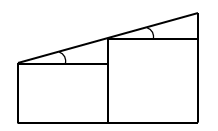
\includegraphics[width=0.4\linewidth]{Text_exercises/Content/pic_2799.png}}
\end{figure}
На рисунке приведен чертеж конструкции крыши. Опоры\newline перпендикулярны уровню земли (горизонту), т.е. $BA\perp AD,$\newline$MN\perp AD, CD\perp AD$. По условию задачи $AN=CD$. Проведем $BP\|AD$ и $MQ\|AD$. Тогда треугольники $BMP$ и $MCQ$ прямоугольные с равными катетами $(BP=AN, MQ=ND=AN)$ и одинаковым острым углом, равным углу наклона крыши к уровню горизонта. Поэтому эти треугольники равны.
Отсюда $MP=CQ$, т.е. $MN-PN=CD-QD$ или $MN-AB=CD-MN$. Таким образом, $AB=2MN-CD=2\cdot2,2-2,5=1,9.$\newline \null \hspace*{\fill} Ответ: 1,9. 

\textbf{2800-2801} Аналогичные задачи.

\textbf{2802.} В формулировке условия задачи имеется неточность. Видимо предполагается, что экран А не просто полностью освещен проектором, но и полностью перекрывает световой поток. В противном случае можно экран А отодвинуть от проектора подальше, и тем не менее он будет полностью освещен. Те же соображения относятся и к экрану В. Поэтому будем эту задачу решать  в предположении, что края экранов находятся на границе светового потока. Тогда решение очевидно: поскольку экран В имеет размер вдвое меньший, чем экран А, его для перекрытия светового потока следует поместить на расстоянии от проектора вдвое меньшем, чем расстояние 300 см, т.е.  на расстоянии 150 см.        \null \hspace*{\fill} Ответ: 150. 

\textbf{2803, 2804.} Аналогичные задачи.

\textbf{2805.} Мальчик шел вдоль катетов прямоугольного треугольника, а расстояние до дома $-$ это длина гипотенузы этого треугольника, т.е. $\sqrt{690^2 + 920^2} = 1150.$ \newline \null \hspace*{\fill} Ответ: 1150. 

\textbf{2806.} Аналогичная задача.

\textbf{2807.} Смещения на запад и восток компенсируют друг друга; можно считать, что девочка сместилась только на север на расстояние 700 м. Именно на таком расстоянии от дома она и оказалась.   \newline \null \hspace*{\fill} Ответ: 700. 

\textbf{2808, 2809} Аналогичные задачи.

\textbf{2810.}
\begin{figure}[h]
\center{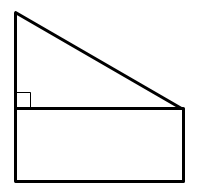
\includegraphics[width=0.4\linewidth]{Text_exercises/Content/pic_2810.png}}
\end{figure}
Будем считать, что сосны растут вертикально,\newline т.е. перпендикулярно к линии горизонта $AC$, при этом $AC=$\newline$=32.$ Отрезками $AB$ и $CD$ изобразим сами сосны с верхушками в точках $B$ и $D$. Проведем $ED\perp AB$. Тогда в прямоугольном треугольнике $BDE, ED=AC=32, BE=AB-AE=$\newline$=AB-CD=37-13=24.$ Расстояние между верхушками $BD=\sqrt{BE^2 + ED^2}=\sqrt{24^2+32^2}=40.$ \newline \null \hspace*{\fill} Ответ: 40. 

\textbf{2811, 2812} Аналогичные задачи.

\textbf{2813.} Пароходы двигаются во взаимно перпендикулярных направлениях. Будем считать, что они двигаются по катетам прямоугольного треугольника, начиная от вершины прямого угла. За 3 часа будут пройдены расстояния $16\text{км/ч}\cdot3\text{ч}=48\text{км и }$\newline$30\text{км/ч}\cdot3\text{ч}=90\text{км .} $ Расстояние между параходами $-$ длина гипотенузы, т.е. $\sqrt{48^2+90^2}=102\text{км.}$ \newline \null \hspace*{\fill} Ответ: 102. 

\textbf{2814-2816.} Аналогичные задачи.

\textbf{2817.}
\begin{figure}[h]
\center{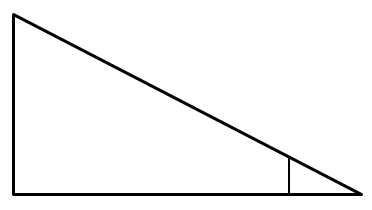
\includegraphics[width=0.4\linewidth]{Text_exercises/Content/pic_2817.png}}
\end{figure}
Пусть $h_1$ и $h_2$ $-$ высота фонаря над уровнем земли и рост\newline человека, $l_1$ $-$ расстояние (по земле) от человека до фонаря, а $l_2$ - длина тени. Из подобия треугольников:
$\frac{h_1}{h_2}=\frac{l_1+l_2}{l_2}$, откуда $h_1=\frac{h_2(l_1+l_2)}{l_2}=\frac{1,6\cdot(18+2)}{2}=16.$ \newline \null \hspace*{\fill} Ответ: 16. 

\textbf{2818-2824.} Аналогичные задачи.

\textbf{2825.}
\begin{figure}[h]
\center{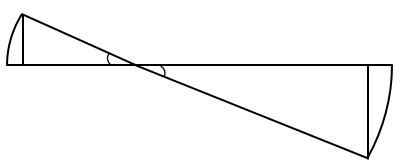
\includegraphics[width=0.4\linewidth]{Text_exercises/Content/pic_2825.png}}
\end{figure}

Пусть $O$ $-$ ось журавля, $l_1$ и $l_2$ $-$ длины его плеч. Если журавля повернуть вокург оси на угол $\alpha$, его короткое плечо поднимется на высоту $h_1=l_1\sin\alpha,$ а длинное $-$ опустится на высоту $h_2=$\newline$=l_2\sin\alpha.$ Таким образом:
$\frac{h_1}{h_2}=\frac{l_1}{l_2}, h_2=\frac{h_1l_2}{l_1}=\frac{0,2\cdot3}{0,5}=1,2.$ \newline \null \hspace*{\fill} Ответ: 1,2. 

\textbf{2826-2832.} Аналогичные задачи.

\textbf{2833.} 
\begin{figure}[h]
\center{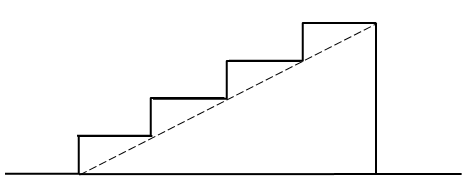
\includegraphics[width=0.4\linewidth]{Text_exercises/Content/pic_2833.png}}
\end{figure}
Пусть число ступеней равно $n$, высота и длина одной ступени равны $h$ и $l$. Тогда расстояние между точками равно:\newline
$n\sqrt{h^2+l^2}=50\cdot\sqrt{14^2+48^2}=2500\text{см}=25\text{м}$ \newline \null \hspace*{\fill} Ответ: 25. 

\textbf{2834-2840.} Аналогичные задачи.

\textbf{2841.} При решении этой и последующих задач \textbf{(2841-2856)} надо принять во внимание следующие соображения. Часовая стрелка делает один оборот $(360^\circ)$ за 12 часов, т.е. за 720 мин., так что  ее угловая скорость движения $\omega=\frac{360}{12\cdot60}=0,5\frac{\text{град}}{\text{мин}}.$ Соответственно, за время $t$ (в минутах) часовая и минутная стрелки поворачиваются на углы $\varphi_1=\omega_1t$ и $\varphi_2=\omega_2t$. Если на циферблате часов имеется 12 цифр, то угловое расстояние между соседними цифрами составляет $\frac{360}{12}=30^\circ$
В частности, в задаче \textbf{2841} в 4 часа минутная стрелка указывает на цифру 12, а часовая $-$ на 4, промежуток между 12 и 4 составляет $4\cdot30=120^\circ$. \newline \null \hspace*{\fill} Ответ: 120. \newline
Или, в задаче \textbf{2845.} $\varphi_2=\omega_2t=6\cdot30=180.$ \newline \null \hspace*{\fill} Ответ: 180. 

\textbf{2857.} $\frac{360^\circ}{5}=72^\circ$ \newline \null \hspace*{\fill} Ответ: 72. 

\textbf{2858-2864.} Аналогичные задачи.

\textbf{2865.} $\frac{11\text{га}}{200\text{м}}=\frac{11\cdot10000\text{кв.м}}{200\text{м}}=559\text{м}$ \newline \null \hspace*{\fill} Ответ: 559. 

\textbf{2866-2868.} Аналогичные задачи.

\textbf{2869.} Пусть $x$ и $4x$ $-$ стороны участка, тогда $4x^2=10000, x=50,$ а периметр $P = 10x = 500.$ \newline \null \hspace*{\fill}Ответ: 500.

\textbf{2870-2873.} Аналогичные задачи.

\textbf{2874.} $\frac{3\cdot5}{0,1\cdot0,25}=600.$ \newline \null \hspace*{\fill} Ответ: 600. 

\textbf{2875-2883.} Аналогичные задачи.

\textbf{2884.} Если ширина окантовки равна $x$ см, то картина с окантовкой имеет площадь $(14+2x)\cdot(19+2x)=696.$ Решив это квадратное уравнение и отбросив отрицательный корень, получим $x=5\text{см}.$ \newline \null \hspace*{\fill} Ответ: 5. 

\textbf{2885-2888.} Аналогичные задачи.

\textbf{2889.} Обозначим через $x$ (см) сторону вырезаемого квадрата. Тогда дно коробки имеет площадь $(55 - 2x)\cdot(36 $-$ 2x)=780$. Решив это уравнение найдем корни $x_1=8, x_2=37,5.$ Второй корень отбрасываем из геометрических соображений. \newline \null \hspace*{\fill} Ответ: 8. 

\textbf{2890-2893.} Аналогичные задачи.

\textbf{2894.} Пусть $x$ и $y$ $-$ длины сторон площадки. Тогда ее площадь равна $xy$, а периметр ограждения $2(x+y).$ Составим систему уравнений:\newline$
\begin{cases}
	2(x+y)=184\\
	xy=2052
\end{cases},
\begin{cases}
	x + y = 92\\
	xy=2052
\end{cases}$
В соответствии с теоремой Виета, неизвестные $x$ и $y$ являются корнями квадратного урванения $t^2 - 92t + 2052 = 0$, т.е. равны 38 и 54. \newline \null \hspace*{\fill} Ответ: 38; 54. 

\textbf{2895-2898.} Аналогичные задачи


\subsection{Статистика}

\textbf{2899.} Содержание жиров (по диаграмме) близко к $10\%$; очень трудно (на глаз) понять, больше или меньше $10\%.$ Мне кажется, что меньше $10\%$, а в ответе дается вариант  $(10-25)\%$.

\textbf{2900.} Самый большой сектор на диаграмме соответствует «прочим» составляющим. \newline \null \hspace*{\fill} Ответ: 4. 

\textbf{2901.} Минимальный сектор соответствует белкам. \newline \null \hspace*{\fill} Ответ: 2. 

\textbf{2902.} Речь идет о «прочих» составляющих. Их явно больше половины, поэтому ответы 1), 3) и 4) явно неверные. \newline \null \hspace*{\fill} Ответ: 2. 

\textbf{2903.} По диаграмме содержание углеводов чуть меньше, чем $25\%$ (четверть круга). Так что ответ 2) сомнителен. Ответ же 3) предполагает, что содержание углеводов примерно $\frac{150}{760}\cdot100\%\approx$\newline$\approx19,7\%$. На глаз это тоже трудно оценить, авторы дают правильный ответ 3).

\textbf{Замечание.} Все задачи с круговыми диаграммами представляют собой достаточно грубую информацию. Правильный ответ можно усмотреть только тогда, когда по диаграмме он совершенно очевиден. К сожалению, не все задачи \textbf{2904-2933} позволяют это сделать. Но тренировать свой глазомер (я даже в подозрительных случаях пользовался транспортиром) и пытаться их все решить, конечно, надо.

\textbf{2934.} Ответ: 2. \textbf{2935.} Ответ: 3. \textbf{2936.} Ответ: 3. \textbf{2937.} Ответ: 4.

\textbf{2938.} Ответ: 4. \textbf{2939.} Ответ: 4. \textbf{2940.} Ответ: 4. \textbf{2941.} Ответ: 3.

 \textbf{2942.} Ответ: 3. \textbf{2943.} Ответ: 2. \textbf{2944.} Ответ: 1, 2.

\textbf{2945.} Ответ: 1,3. 

\textbf{2946-2953.} Аналогичные задачи.

\textbf{2954.} Ответ: 3; 4.

\textbf{2955-2958.} Аналогичные задачи.

\subsection{Теория вероятностей}

\textbf{2959.} Трехзначные числа $-$ это числа от 100 до 999. Всего их $n=$\newline$=900.$ Делятся на 100 $m=9$ чисел: 100, 200, ..., 900. По формуле классической вероятности: $P=\frac{m}{n}=\frac{9}{900}=0,01.$ \newline \null \hspace*{\fill} Ответ: 0,01. 

\textbf{2960.} Аналогичная задача.

\textbf{2961.} Как и в задаче \textbf{2959}, $n=900$. На 11 делятся числа вида $99+11k, k=1, 2, \dots, m.$ Чтобы найти $m$, надо решить неравенство $99+11m\leq999, 11m\leq900.$ Очевидно, $m=\bigg[\frac{900}{11}\bigg]=81.$ В математике символ $[x]$ обозначает целую часть числа $[x]$, т.е. максимальное целое число, не превосходящее $x$. Таким образом, $P = \frac{m}{n}=\frac{81}{900}=0,09.$ \newline \null \hspace*{\fill} Ответ: 0,09. 

\textbf{2962-2990.} Аналогичные задачи.

\textbf{2991.} Если $A$ и $\overline{A}$ $-$ два противоположных события, то $P(A)+$\newline$+P(\overline{A})=1,$ т.е. по известной вероятности события легко вычисляется вероятность противоположного события. В нашем случае $P = 1 - 0,06 = 0,94.$ \null \hspace*{\fill} Ответ: 0,94. 

\textbf{2992, 2993.} Аналогичные задачи.

\textbf{2994.} $n=206,\enspace m=20+\frac{206-20-8-12}{2}=20+83=103,\enspace P=\frac{103}{206}=$\newline$=0,5.$ \newline \null \hspace*{\fill} Ответ: 0,5. 

\textbf{2995, 2996} Аналогичные задачи.

Задачи \textbf{2997-3001} решаются по формуле классической вероятности; надо четко подсчитать общее число исходов $n$ и число благоприятных исходов $m$.

\textbf{3002.} Бросать две монеты одновременно, последовательно или одну и ту же монету два раза $-$ вопрос совершенно не принципиальный. Если монета симметричная, то выпадение герба (орла) или решки (решетки) $-$ события равновозможные, вероятность каждого из них при однократном бросании равна 0,5. При двух бросаниях возможно 4 исхода эксперимента: РР, РГ, ГР, ГГ (Р и Г $-$  появление решки и герба. Благоприятным является один исход ГГ. Поэтому $P = \frac{m}{n}=\frac{1}{4}=0,25.$ \newline \null \hspace*{\fill} Ответ: 0,25. 

\textbf{3003.} Благоприятными исходами являются РГ и ГР, так что $P = \frac{m}{n} =\frac{2}{4} = 0,5.$ \newline \null \hspace*{\fill} Ответ: 0,5. 

\textbf{3004.} Возможные исходы: РРР, РРГ, РГР, РГГ, ГРР, ГРГ, ГГР, ГГГ. Всего таких исходов $n=2^3=8$ Благоприятных исход один: ГГГ. $P = \frac{1}{8} = 0,125.$ \newline \null \hspace*{\fill} Ответ: 0,125. 

\textbf{3005.} Благоприятных исхода три: РГГ, ГРГ, ГГР. $P=\frac{3}{8}=0,375.$ \newline \null \hspace*{\fill} Ответ: 0,375. 

\textbf{3006.} Если Петя оказался в какой-либо группе, то для Кости осталось всего 19 вакансий: 15 мест в тех трех группах, куда Петя не попал, и 4 места в той группе, где оказался Петя. Таким образом, из $n=19$ возможных вариантов только m=4 являются благоприятными. Поэтому $P=\frac{m}{n}=\frac{4}{19}.$ \newline \null \hspace*{\fill} Ответ: $\frac{4}{19}.$ 

\textbf{3007.} Аналогичная задача.

\textbf{3008.} Это аналог задачи \textbf{2003}. \null \hspace*{\fill} Ответ: 0,5. 

\textbf{3009.} Аналог задачи \textbf{3004}.\newline \null \hspace*{\fill} Ответ: 0,375. 

\textbf{3010.} В соревнованиях всего участвует 6+4+3+7=20 спортсменов. Последним может оказаться с равными возможностями каждый из участников. Таким образом, всего существует $n=20$ вариантов последней позиции в списке участников. Из них «благоприятных» (соответствующих заданному вопросу) $-$ $m=7$, по числу участков из Венгрии. Тогда $P = \frac{m}{n}=\frac{7}{20}=0,35.$\newline \null \hspace*{\fill} Ответ: 0,35. 

\textbf{3011-3013.} Аналогичные задачи.

\textbf{3014} При бросании двух игральных костей возможны следующие 36 исходов (первая цифра означает число очков на первой кости, втора $-$ на другой):
\begin{center}$
\begin{matrix}
11& 12& 13& 14& 15& 16&\\
21& 22& 23& 24& 25& 26&\\
31& 32& 33& 34& 35& 36&\\
41& 42& 43& 44& 45& 46&\\
51& 52& 53& 54& 55& 56&\\
61& 62& 63& 64& 65& 66&\\
\end{matrix}$
\end{center}
Эти исходы являются равновозможными, несовместными и образуют полную группу событий. Именно в такой ситуации следует использовать формулу классической вероятности. Таким образом, $n=36.$
Нас интересует событие, заключающееся в том, что в сумме выпадает 9 очков. Благоприятные исходы (см. таблицу): 36, 45, 54, 63, т.е. $m=4$. Поэтому $P = \frac{m}{n}=\frac{4}{36}=\frac{1}{9}\approx0,11.$ \newline \null \hspace*{\fill} Ответ: 0,11. \newline
\textbf{3015-3017.} Аналогичные задачи.\newline
\textbf{3018.} Рассмотрим следующие события\newline$A$ $-$ школьнику досталась задача по теме «Треугольники»;\newline$B$ - школьнику досталась задача по теме «Окружность».\newline События $A$ и $B$ $-$ несовместные, т.к. задач, которые одновременно относятся к этим темам, в сборнике нет. Нас интересует вероятность суммы этих событий, т.е. $P(A+B)$. Суммой событий называется события, состоящее в том, что наступило $A$ или $B$.\newline Для несовместных событий: $P(A+B)=P(A)+P(B)=0,5+\linebreak+0,25=0,75.$\null \hspace*{\fill} Ответ: 0,75. 

\textbf{3019-3021.} Аналогичные задачи.

\textbf{3022.} Рассмотрим следующие события:\newline $A$ $-$ при первом выстреле стрелок попал в мишень;\newline$B$ $-$ при втором выстреле стрелок попал в мишень;\newline$C$ $-$ при третьем выстреле стрелок попал в мишень;\newline$D$ $-$ при четвертом выстреле стрелок промахнулся.\newline При этом $P(A)=P(B)=P(C)=P(D)=0,5.$\newline Нас интересует вероятность того, что все эти события произошли, т.е. вероятность произведения событий $P(ABCD)$. Указанные события никак между собой не связаны, т.е. независимы. В этом случае $P(ABCD)=P(A)P(B)P(C)P(D)=0,5^4=0,0625.$ \newline \null \hspace*{\fill} Ответ: 0,0625. 

\textbf{3023-3029.} Аналогичные задачи.

Задачи \textbf{3030-3033} решаются на основе формулы классической вероятности.

\textbf{3034.} Обозначим через $T$ срок безотказной работы компьютера (в годах). Поусловию задачи $P(T>1)=0,98$, а $P(T>2)=0,84.$ Нас интересует $P(1<T<2)$.\newline Очевидно, $P(T<1)=1-0,98=0,02$, а $P(T<2)=1-0,84=$\newline$=0,16$. Но $P(T<2)=P(T<1)+P(1<T<2)$, так что \newline$P(1<T<2)=P(T<2)-P(T<1)=0,16-0,02=0,14.$ \newline \null \hspace*{\fill} Ответ: 0,14. 

\textbf{Замечание.} Строгие знаки неравенств в решении задачи \textbf{3034} не должны смущать. Вероятность того, что непрерывная случайная величина принимает какое-либо конкретное значение, в теории вероятностей считается равной нулю. Поэтому, например, $P(T<1)=P(T\leq1)$ или $P(1<T<2)=P(1\leq T\leq2)$ и т.д.

\textbf{3035-3037} Аналогичные задачи.

\textbf{3038} В данном случае $n=39-24=15, m=3$ (из заданных чисел на 5 делятся 25, 30 и 35). Поэтому $P=\frac{m}{n}=\frac{3}{15}=0,2$ \newline \null \hspace*{\fill} Ответ: 0,2. 

\textbf{3039-3041.} Аналогичные задачи.

\textbf{3042.} $n=450,\enspace m=450-2\cdot180=90,\enspace P=\frac{90}{450}=0,2.$ \newline \null \hspace*{\fill} Ответ: 0,2. 

\textbf{3043-3045.} Аналогичные задачи.

\textbf{3046.} Пусть $M$ $-$ число задач предлагаемых при тестировании, а $k$ $-$ число решенных учащимся задач. Тогда
\begin{eqnarray*}
	P(k>11)=P(k=12)+P(k=13)+\dots+P(k=M),\\
	P(k>10)=P(k=11)+P(k=12)+\dots+P(k=M).
\end{eqnarray*}
Вычтем из второго равенства первое, получим:
\begin{eqnarray*}
	P(k>10)-P(k>11)=P(k=11), \text{откуда получаем}\\
	P(k=11)=P(k>10)-P(k>11)=0,71-0,65=0,06.
\end{eqnarray*}
\newline \null \hspace*{\fill} Ответ: 0,06. 

\textbf{3047-3049.} Аналогичные задачи.

\textbf{3050.} Пусть $k$ - случайное число пассажиров в автобусе. По условию задачи $P(k<22)=0,86;\enspace P(k<9)=0,5.$\newline Тогда $P(9\leq k\leq21)=P(k<22)-P(k<9)=0,86-0,5=0,36.$ \newline \null \hspace*{\fill} Ответ: 0,36. 

\textbf{3051-3053.} Аналогичные задачи.

\textbf{3054.} Эта задача легко решается с помощью \textbf{формулы полной вероятности}. Простейший вариант формулы полной вероятности выглядит так: если есть две гипотезы $H_1$ и $H_2$, вероятности которых $P(H_1)$ и $P(H_2)$ известны (при этом $P(H_1) + P(H_2)=1$) и некоторое событие $A$, которое может наступить только в результате наступления одного из событий $H_1$ или $H_2$, то полная вероятность события $A$ вычисляется по формуле: \newline$P(A)=P(H_1)P(A|H_1)+P(H_2)P(A|H_2)$, где $P(A|H_i)(i=1,2)$ $-$ так называемые \textbf{условные} вероятности события $A$, вычисленные в предположении, что события $H_i$ уже наступили. В более сложном варианте гипотез не две, а $n$ и в формулу полной вероятности входит не два, а $n$ слогаемых. В нашем случае гипотезы две:\newline $H_1$ $-$ выбранная дл контроля батарейка исправная $(P(H_1)=$\newline$=0,95)$;\newline$H_2$ $-$ выбранная для контроля батарейка неисправная $(P(H_2)=$\newline$=0,05).$
Через $A$ обозначим событие: случайно выбранная батарейка системой контроля забракована. Условные вероятности : $P(A|H_1)=0,03;\newline P(A|H_2)=0,99.$\newline Тогда по формуле полной вероятности $P(A)=P(H_1)P(A|H_1)+$\newline$+P(H_2)P(A|H_2)=0,95\cdot0,03+0,05\cdot+0,99=0,078.$ \newline \null \hspace*{\fill} Ответ: 0,078. 


\textbf{3054-3057.} Аналогичные задачи.

\chapter*{ПРИЛОЖЕНИЕ}
\addcontentsline{toc}{chapter}{ПРИЛОЖЕНИЕ}
\subsection*{Таблица решенных задач}
\begin{table}[H]
\begin{center}
\begin{tabular}{|c|c|c|c|}
\hline
~ & ~ & Номера & ~ \\
№ & Наименование & задач в & Номера\\
раздела & раздела & сборнике & решенных\\
~ & ~ & И.В. & задач \\
~ & ~ & Ященко & \\
\hline
1.1.1 &Натуральные числа& 1-10 (10) & 1 - 10\\
\hline
~ & ~ & ~ & 11-100,\\
1.1.2 & Рациональные & 11-137 & 102,103,107,110,\\
~ & числа & (127) & 112,115,118,124,\\
~ & ~ & ~ & 128,130,132,136\\
\hline
~ & ~  & ~ & 138,141,147,\\
1.1.3 & Действительные & 138-172 & 149,150,153,\\
~ & числа & (34) & 158,163,168\\
\hline
~ & ~ & ~ & 173,174,179,184,\\
1.2.1 & Буквенные & 173-225 & 186,194,197,\\
~ & выражения & (52) & 200,204,208,\\
~ & ~ & ~ & 215,219,224\\
\hline
~ & ~ & ~ & 226,230,234,\\
1.2.2 & Многочлены & 226-295 & 238,242,244,248,\\
~ & ~ & (69) & 252,256,260,272,\\
~ & ~ & ~ & 276,284,295\\
\hline
~ & ~ & ~ & 296-299,305,311,\\
~ & ~ & ~ & 317,320,326,333,\\
~ & ~ & ~ & 338,343,346,347,\\
1.2.3 & Алгебраические & 296-478 & 351,355,356,362,\\
~ & дроби & (183) & 366,368,372,377,\\
~& ~ & ~ & 381,384,392,395,\\
~ & ~ & ~ & 398,401,432,436,\\
~ & ~ & ~ & 440,446,452,456,\\
~ & ~ & ~ & 459,461,462,466,\\
~ & ~ & ~ & 472,476,478\\
\hline
\end{tabular}
\end{center}
\end{table}

\begin{table}[H]
\begin{center}
\begin{tabular}{|c|c|c|c|}
\hline
~ & Степени с целыми & 479-513 & 479,482,485,488,492,\\
1.2.4 & показателями и их & (35) & 496,499,502,506,510,\\
~ & свойства & ~ & 513\\
\hline
~ & ~ & ~ & 514,517,521,526,528,\\
~ & ~ & ~ & 529,532,535,540,543,\\
1.2.5 & Квадратный корень & 514-582 & 546,548,549,550,555,\\
~ & и его свойства & (69) & 558,560,563,567,570,\\
~ & ~ & ~ & 573,574,577,580,582\\
\hline
~ & Линейные & 583-769 & 583,614,701,\\
1.3.1 & уравнения с одной & (187) & 723,747,756,\\
~ & переменной & ~ & 769\\
\hline
1.3.2 & Квадратные & 770-816 & 770,775,778,779,783,\\
~ & уравнения & (47) & 797,805,814\\
\hline
1.3.3 & Рациональные & 817-863 & 817,827,832,841,851,\\
~ & уравнения & (47) & 858\\
\hline
~ & Системы двух & 864-879 & 864,865,\\
1.3.4 & уравнений с двумя & (16) & 868,872,\\
~ & переменными & ~ & 874,878\\
\hline
~ & Числовые & 880-914 & 880,881,883,885,889,\\
1.3.5 & неравенства и их & (35) & 890,895,897,900,902,\\
~ & свойства & ~ & 907,908,911\\
\hline
~ & Линейные & 915-1118 & 915,921,930,\\
1.3.6 & неравенства с одной & (204) & 934,938,939,\\
~ & переменной & ~ & 945,955\\
\hline
~ & Системы линейных & 1119-1133 & 1119,1123,\\
1.3.7 & неравенств с одной & (15) & 1126,\\
~ & переменной & ~ & 1129\\
\hline
~ & ~ & ~ & 1134,1144,1149,1154,\\
1.3.8 & Квадратные & 1134-1264 & 1159,1164,1169,1174,\\
~ & неравенства & (131) & 1188,1203,1206,1218,\\
~ & ~ & ~ & 1234,1261\\
\hline
1.4.1 & Последовательности & 1265-1290 & 1265,1270,1272,\\
~ & ~ & (26) & 1275,1280,1286\\
\hline
~ & Арифметическая & 1291-1361 & 1291,1301,1306,1311,\\
1.4.2 & прогрессия & (71) & 1321,1326,1331,1336,\\
~ & ~ & ~ & 1341,1346,1351,1357\\
\hline
~ & Геометрическая & 1362-1411 & 1362,1347,1372,1376,\\
1.4.3 & прогрессия & (500) & 1381,1386,1396,1402,\\
~ & ~ & ~ & 1408\\
\hline
\end{tabular}
\end{center}
\end{table}


\begin{table}[H]
\begin{center}
\begin{tabular}{|c|c|c|c|}
\hline
~ & Линейная, & ~ & 1412,1413,1420,1428,\\
1.5.1 & квадратичная, & 1412-1505 & 1434,1440-1444,\\
~ &  обратно & (94) & 1448,1451,1454,\\
~ & пропорциональные & ~ & 1460,1472-1475,\\
~ & функции & ~ & 1484,1496\\
\hline
~ & Графическая & ~ & 1506,1510,1514,1518,\\
~ & интерпретация & ~ & 1522,1526,1534-1538,\\
1.5.2 & уравнений, & 1506-1614 & 1542,1546,1550,\\
~ & неравенств и & (109) & 1562-1570,1574-1578,\\
~ & их систем & ~ & 1586,1587,1590,1594,\\
~ & ~ & ~ & 1598,1602,1610\\
\hline
~  & Основные понятия & 1615-1644 & ~\\
2.1 & и утверждения & (30) & 1615-1644\\
~ & геометрии & ~ & ~\\
\hline
~ & Геометрия & 1645-1694 & 1645-1649,1655,1660,\\
2.2  & на клетчатой & (50) & 1665,1670,1675,1680,\\
~ & бумаге & ~ & 1685,1690\\
\hline
~ & ~ & ~ & 1695,1698,1701,1704,\\
~ & ~ & ~ & 1710,1713,1716,1718,\\
~ & ~ & ~ & 1728,1736,1744,1750,\\
~ & ~ & ~ & 1756,1760,1765,1768,\\
2.3 & Треугольники & 1695-1846 & 1772,1776,1780, 1784,\\
~ & ~ & (152) & 1788,1792,1794,1796,\\
~ & ~ & ~ & 1802,1803,1807,1808,\\
~ & ~ & ~ & 1811,1815,1819,1827,\\
~ & ~ & ~ & 1831,1835,1839\\
\hline
~ & ~ & ~ & 1847,1850,1853,1856,\\
~ & ~ & ~ & 1859,1862,1856,1868,\\
~ & ~ & ~ & 1871,1874,1877,1880,\\
~ & ~ & ~ & 1883,1887,1891,1895,\\
~ & ~ & ~ & 1901,1905,1909,1913,\\
2.4 & Четырехугольники & 1847-2016 &1917,1925,1929,1933,\\
~ & ~ & (170) & 1937,1941,1945,1949,\\
~ & ~ & ~ & 1953,1957,1965,1969,\\
~ & ~ & ~ & 1973,1977,1981,1985,\\
~ & ~ & ~ & 1989,1993,1997,2001,\\
~ & ~ & ~ & 2005,2009,2013\\
\hline
\end{tabular}
\end{center}
\end{table}
\begin{table}[H]
\begin{center}
\begin{tabular}{|c|c|c|c|}
\hline
~ & ~ & ~ & 2017,2020,2023,2026,\\
~ & ~ & ~ & 2029,2032,2035,2038,\\
~ & ~ & ~ & 2041,2044,2050,2056,\\
~ & ~ & ~ & 2062,2068,2074,2077,\\
~ & ~ & ~ & 2080,2083,2086,2092,\\
~ & ~ & ~ & 2098,2104,2107,2110,\\
2.5 & Окружность и круг & 2017-2221 & 2113,2119,2122,2125,\\
~ & ~ & (205) & 2128,2131,2134,2137,\\
~ & ~ & ~ & 2143,2146,2149,2151,\\
~ & ~ & ~ & 2154,2157,2160,2163,\\
~ & ~ & ~ & 2166,2169,2172,2175,\\
~ & ~ & ~ & 2178,2181,2184,2187,\\
~ & ~ & ~ & 2190,2193,2196,2199,\\
~ & ~ & ~ & 2202,2210,2214,2218\\
\hline
~ & ~ & ~ & 2222,2227,2230,2233,\\
2.6 & Тригонометрия & 2222-2321 & 2234,2236,2242,2246,\\
~ & ~ & (100) & 2250,2254,2258,2262,\\
~ & ~ & ~ & 2282,2290,2304,2306\\
\hline
~ & ~ & ~ & 2322,2323,2327,2332,\\
~ & Векторы на & 2232-2421 & 2342,2347,2352,2357,\\
2.7 & плоскости & (100) & 2362,2367,2372,2377,\\
~ & ~ & ~ & 2382,2387,2392,2407,\\
~ & ~ & ~ & 2412,2417\\
\hline
~ & ~ & ~ & 2422,2425,2427,2432,\\
~ & ~ & ~ & 2437,2442,2447,2452,\\
~ & ~ & ~ & 2457,2462,2467,2471,\\
~ & ~ & ~ & 2475,2479,2483,2486,\\
~ & ~ & ~ & 2489,2492,2495,2499,\\
~ & ~ & ~ & 2503,2507,2511,2515,\\
3.1 & Текстовые задачи & 2422-2631 & 2519,2523,2527,2531,\\
~ & ~ & (210) & 2535,2541,2547,2550,\\
~ & ~ & ~ & 2554,2558,2562,2566,\\
~ & ~ & ~ & 2570,2574,2578,2582,\\
~ & ~ & ~ & 2586,2590,2594,2598,\\
~ & ~ & ~ & 2602,2612,2617,2622,\\
~ & ~ & ~ & 2627\\
\hline
\end{tabular}
\end{center}
\end{table}
\begin{table}[H]
\begin{center}
\begin{tabular}{|c|c|c|c|}

\hline
~ & Представление & ~ & 2632,2635,2638,2644,\\
3.2 & зависимостей между & 2632-2697 & 2647,2650,2653,2656,\\
~ & величинами в виде & (66) & 2659,2662,2675,2678,\\
~ & формул & ~ & 2682,2686,2690,2694\\
\hline
~ & Чтение графиков & 2698-2789 & 2698-2702,2748-2755,\\
3.3 & реальных & (92) & 2760-2763,2768,2772,\\
~ & зависимостей & ~ & 2776,2777,2780-2784\\
\hline
~ & ~ & ~ & 2790,2799,2802,2805,\\
~ & ~ & ~ & 2807,2810,2813,2817,\\
3.4 & Прикладные задачи & 2790-2897 & 2825,2833,2841,2845,\\
~ & по геометрии & (108) & 2857,2865,2869,2874,\\
~ & ~ & ~ & 2884,2889,2894\\
\hline
3.5 & Статистика & 2899-2958 & 2899-2903,2934-2945,\\
~ & ~ & (60) & 2954\\
\hline
~ & ~ & ~ & 2959,2961,2991,2994,\\
~ & Теория & 2959-3057 & 3002-3006,3008,3009,\\
3.6 & вероятностей & (99) & 3010,3014,3018,3022,\\
~ & ~ & ~ & 3034,3038,3042,3046,\\
~ & ~ & ~ & 3050,3054\\
\hline
\end{tabular}
\end{center}
\end{table}



